\documentclass[11pt,letterpaper]{article}
\usepackage{macroshw}

\title{\begin{spacing}{1.2}Quantum Mechanics I\\HW 5\end{spacing}}
\author{Matthew Phelps}
\date{Due: April 9}

\begin{document}
\maketitle

\benum
% #1 --------------------------------------------------------------------------------------------------------------------------------------------------------------------------------------
  	\item 
	
	\benum
		% (a)
		\item 
		Given the usual eigenstates $\ket{j,m}$ of the angular momentum operators $\vect J^2$ and $J_z$, determine the expectation 
		values $\braket{j,m|J_x|j,m}$ and $\braket{j,m|J_y|j,m}$.
		\\ 
		\\
		Since we cannot compute these expectation values directly, we must either expand the states in terms of $J_{x,y}$ eigenstates
		or we must express $J_{x,y}$ in terms of something else we know. The latter can be done via the ladder operators defined as
		\[
			J_\pm \equiv J_x\pm iJ_y
		\]
		\[
			J_\pm \ket{j,m} = \sqrt{(j\mp m)(j\pm m+1)}\h\ket{j,m\pm 1}.
		\]
		For $J_x$ and $J_y$ we have
		\[
			J_x = \frac 12 \plr{J_++J_-};\quad J_y  = -\frac{i}{2} \plr{J_+-J_-}.
		\]
		Taking the expectation value for $J_x$ we have 
		\ba
			\braket{j,m|J_x|j,m} &= \frac 12\braket{j,m|J_++J_-|j,m} \\
			&= \frac{1}{2}\braket{j,m|J_+|j,m}+\frac 12\braket{j,m|J_-|j,m}\\
			& = \frac{\h}{2}\sqrt{(j-m)(j+m+1)}\braket{j,m|j,m+1}\\
			&\quad +\frac{\h}{2}\sqrt{(j+m)(j-m+1)}\braket{j,m|j,m-1}
		\ea
		As Hermitian operators, the eigenstates of $J_z$ and $\vect J^2$ are orthogonal
		\[
			\braket{j,m|j',m'} = \delta_{j,j'}\delta_{m,m'}
		\]
		thus we have 
		\[
			\braket{j,m|J_x|j,m} = \braket{j,m|J_y|j,m} = 0.
		\]
		\\
		
		% (b)
		\item 
		Find the standard deviation $\Delta J_i = \sqrt{\braket{j,m|J_i^2|j,m}-\braket{j,m|J_i|j,m}^2}$ for $J_x$ and $J_y$. 
		\\
		\\
		Since the second term is zero, the standard deviation amounts to finding $\blr{\braket{j,m|J_i^2|j,m}}^{1/2}$ for $J_x$
		and $J_y$. Start with
		\[
			J_x^2 = \frac{1}{4}(J_+^2+J_-^2+J_+J_-+J_-J_+)
		\]
		\[
			J_y^2 = -\frac{1}{4}(J_+^2+J_-^2-J_+J_--J_-J_+),	
		\]
		then form the expectation values
		\ba
			\braket{j,m|J_x^2|j,m} &= \frac 14\braket{j,m|(J_+^2+J_-^2+J_+J_-+J_-J_+)|j,m}\\
			&  = \frac{1}{4}\braket{j,m|J_+J_-+J_-J_+|j,m} 
		\ea
		\ba
			\braket{j,m|J_y^2|j,m} &= -\frac 14\braket{j,m|(J_+^2+J_-^2-J_+J_--J_-J_+)|j,m}\\
			&  = \frac{1}{4}\braket{j,m|J_+J_-+J_-J_+|j,m} .
		\ea
		Applying orthogonality, we see that the expectation values are the same. Before we continue, it is helpful to notice that
		\[
			J_+J_- = J_x^2+J_y^2-i[J_x,J_y] = \vect J^2-J_z^2+\h J_z
		\]
		\[
			J_-J_+ = J_x^2+J_y^2+i[J_x,J_y] = \vect J^2-J_z^2-\h J_z.
		\]
		The expectation values are now easily calculated as 
		\[
			\braket{j,m|J_x^2|j,m} = \braket{j,m|J_y^2|j,m}=\frac{1}{2}\blr{j(j+1)\h^2-m^2\h^2)}.
		\]
		The standard deviation is then
		\[
			\Delta J_x = \Delta J_y = \frac{\h}{\sqrt 2}\sqrt{j(j+1)-m^2}
		\]
		\\
		
		% (c)
		\item
		Determine the eigenvalues and construct the \emph{real} eigenfunctions of the Hamiltonian involving orbital angular
		momentum of a single particle, $H = a(L_x^2+L_y^2)+bL_z^2$, where $a\ne b$ are real constants. \\ \\
		Possibly helpful identity: $Y^*_{l,m}(\theta,\phi) = (-1)^mY_{l,-m}(\theta,\phi)$. 
		\\
		\\
		\\
		As an aside, this is the Hamiltonian corresponding to a symmetric rigid rotor (or top), which has application to rotational 
		spectroscopy. The coefficients are related to the moments of inertia and since $a\ne b$, we have a prolate or oblate rotor. We 
		may first rewrite our Hamiltonian as
		\[
			H = a\vect L^2 +(b-a)L_z^2
		\]
		in which we see that
		\[
			[H,\vect L^2] = [H, L_z] = 0.
		\]
		It is clear that the energy eigenfunctions are simultaneous eigenfunctions of $\vect L^2$ and $L_z$, i.e.
		\[
			H\ket{E,l,m} = E\ket{E,l,m}
		\]
		\[
			\vect L^2\ket{E,l,m} = l(l+1)\h^2 \ket{E,l,m}
		\]
		\[
			L_z\ket{E,l,m} = m\h\ket{E,l,m}
		\]
		Immediately, we can find the energy spectrum of the Hamiltonian
		\[
			H\ket{E_n,l,m} = l(l+1)a\h^2 +(b-a)\h^2m^2\ket{E,l,m}.
		\]
		Being orbital angular momentum, we know that $l$ must take on integer values (multiple reasons listed on Sakurai
		p. 204, single-valuedness being one of the most apparent) and that $m$ ranges from $[-l,l]$ in integer steps. Therefore, our 	
		energy eigenvalues are twofold degenerate ($\pm m)$. As for the wavefunction, we know that the spherical harmonics 
		simultaneously represent the eigenfunctions of both $\vect L^2$ and $L_z$:
		\[
			\braket{\vecth n|L_z|l,m} = m\h\braket{\vecth n|l,m}= -i\h\pdiff\phi\braket{\vecth n|l,m} 
		\]
		\[
			-ih\pdiff\phi Y_l^m(\theta,\phi) = m\h Y_l^m(\theta,\phi)
		\]
		and
		\[
			\braket{\vecth n|\vect L^2|l,m} = l(l+1)\braket{\vecth n|l,m}
		\]
		\[
			 -\h^2\blr{\frac{1}{\sin\theta}\pdiff\theta\plr{\sin\theta\pdiff\theta}+\frac{1}{\sin^2\theta}\pdifff{}{*2\phi}}
			Y_l^m(\theta,\phi)=\h^2l(l+1)Y_l^m(\theta,\phi)
		\]
		where the spherical harmonics for $m\ge 0$ can be written as
		\[
			Y_l^m(\theta,\phi) = (-1)^mNe^{im\phi}P_l^m(\cos\theta)
		\]
		in which we denote for brevity
		\[
			N = \sqrt{\frac{(2l+1)(l-m)!}{4\pi(l+m)!}}.
		\]
		This normalization factor differs slightly from that in Sakurai p. 204 but both can be shown to be 	
		equivalent under appropriate usage. For $m<0$ we simply use the relation
		\be\label{1}
			Y^{-m}_l(\theta,\phi) = (-1)^m(Y_l^m)^*.
		\ee
		Since the associated Legendre polynomials are real, the only complex argument in the spherical harmonics comes from
		$e^{im\phi}$. To express a complex phase in a real basis, the most natural choice of basis is that of sine and cosine. As a first 
		step, it may be useful to note that we can express our complex spherical harmonic solutions in pieces as
		\[
			Y_l^m = \begin{cases} \ds  \sqrt{\frac{(2l+1)(l-|m|)!}{4\pi(l+|m|)!}}e^{im\phi}P_l^{|m|}(\cos\theta) &\quad m<0\\ \\
			\ds \sqrt{\frac{2l+1}{4\pi}}P_l(\cos\theta)&\quad m=0\\ \\
			\ds 	(-1)^m\sqrt{\frac{(2l+1)(l-m)!}{4\pi(l+m)!}}e^{im\phi}P_l^m(\cos\theta)  &\quad m>0.
			\end{cases}
		\]
		Following this layout, if we choose the spherical harmonics to be sine and cosine functions, then we can construct a real
		orthonormal basis as 
		\[
			\tilde Y_l^m = \begin{cases} \ds  \frac{i}{\sqrt 2}\plr{Y_l^m-Y^{*m}_l}&\quad m<0\\ \\
			\ds Y_l^0&\quad m=0\\ \\
			\ds  \frac{1}{\sqrt 2}\plr{Y_l^m+Y^{*m}_l}&\quad m>0.
			\end{cases}
		\]
		Since cosine is even in $m$, it would not be appropriate to include in the definition for $m<0$. In addition, any real even or odd 
		function of spherical harmonics can now easily be composed by choosing appropriate terms with $m>0$ (even) or $m<0$ (odd).
		Using \eqref{1} we can express the real spherical harmonic basis alternatively as
		\[
			\tilde Y_l^m = \begin{cases} \ds  \frac{i}{\sqrt 2}\plr{Y_l^m-(-1)^mY^{-m}_l}&\quad m<0\\ \\
			\ds Y_l^0&\quad m=0\\ \\
			\ds  \frac{1}{\sqrt 2}\plr{Y_l^{m}+(-1)^mY^{m}_l}&\quad m>0.
			\end{cases}
		\]
		The real spherical harmonics have a $\phi$ dependence that is proportional to sine or cosine. As such, they are 
		\emph{not} eigenfunctions of $L_z$. However, they are eigenfunctions of $L_z^2$, which is what we need from 
		our Hamiltonian. Since $\vect L^2$ is also proportional to $\pdifff{}{*2\phi}$ the eigenvalues of $\vect L^2$ remain unchanged 
		and thus we find that the real spherical harmonics serve as eigenfunctions of our Hamiltonian. In summary
		\[
			E_{lm}= l(l+1)a\h^2 +(b-a)\h^2m^2\quad (l\in \mathbb{Z},\ m=-l,-l+1\  ...\  l-1,l)
		\]
		\[
			\psi_{lm}(\theta,\phi) = \tilde Y_l^m(\theta,\phi) = \begin{cases} \ds  \frac{i}{\sqrt 2}\plr{Y_l^m-(-1)^mY^{-m}_l}&\quad m<0\\ \\
			\ds Y_l^0&\quad m=0\\ \\
			\ds  \frac{1}{\sqrt 2}\plr{Y_l^{m}+(-1)^mY^{m}_l}&\quad m>0.
			\end{cases}
		\]
		\\
		\\
		\eenum
		
	
% #2 ------------------------------------------------------------------------------------------------------------------------------------------------------------------
	\item
	Consider measurement of a spin 1/2 in the direction $\vecth n = \cos\alpha \vecth e_x+\sin\alpha\vecth e_z$, so that
	we are measuring the operator $S(\alpha)$ with the corresponding normalized eigenvectors $\xi_\pm(\alpha)$,
	\[
		S(\alpha) = \frac{\h}{2}
		\begin{pmatrix} \cos\alpha&\sin\alpha\\\sin\alpha &-\cos\alpha
		\end{pmatrix}
	\]
	\[
		\xi_+(\alpha) = \begin{pmatrix}\cos \frac \alpha2 \\ \sin \frac \alpha2 \end{pmatrix};\quad
		\xi_-(\alpha) = \begin{pmatrix}-\sin\frac \alpha2 \\ \cos \frac \alpha 2 \end{pmatrix}.
	\]	
		\benum
		% (a)
		\item
		Suppose you prepare the system initially in the state $\xi_+(0)$, then measure successively in the directions $\alpha$, $2
		\alpha$, ..., $n\alpha$. Show that the probability that the result is $+\h/2$ every time is $\plr{\cos \frac \alpha2}^{2n}$.
		\\
		\\
		Straying a little from the spinor formalism, we can represent the spinor
		$\xi_+(0)$ as
		\ba
			\ket{\xi_+(0)} &= \blr{\cos\frac02 \ket{+} +\sin\frac02 \ket -} \\
			&= \ket +\\
			& = \ket{\xi_+(\alpha)}\braket{\xi_+(\alpha)|+}+\ket{\xi_-(\alpha)}\braket{\xi_-(\alpha)|+}.
		\ea
		Applying $S(\alpha)$ then collapses the state into either of its eigenkets with respective probabilities 
		$\braket{\xi_\pm(\alpha)|+}$. The probability of obtaining $\h/2$ from a measurement $S(\alpha)$ onto $\xi_+(0)$ is therefore
		\[
			\braket{\xi_+(\alpha)|+} = \begin{pmatrix}\cos\frac\alpha2&\sin\frac\alpha2\end{pmatrix}
			\begin{pmatrix}1\\0\end{pmatrix} = \cos\frac\alpha2.
		\]
		After measurement the state is known to be in $\xi_+(\alpha)$. A subsequent measurement of $S(2\alpha)$ can be seen to have
		a probability of obtaining $\h/2$ as
		\ba
			\braket{\xi_+(2\alpha)|\xi_+(\alpha)} &= \xi_+^\dag(2\alpha)\xi_+(\alpha)\\
			 &= \begin{pmatrix}\cos\alpha&\sin\alpha\end{pmatrix}
			\begin{pmatrix}\cos\frac\alpha2\\\sin\frac\alpha2\end{pmatrix}\\
			& = \cos\alpha\cos\frac\alpha2+\sin\alpha\sin\frac\alpha2\\
			& = \cos\plr{\alpha-\frac\alpha2}\\
			& = \cos\frac\alpha2.
		\ea	
		As all measurements are separated by $\alpha$ we can see that the probability of obtaining $\h/2$ after an individual 
		measurement is
		\[
			\xi_+^\dag(n\alpha)\xi_+((n-1)\alpha) = \cos\frac\alpha2.
		\]
		After $n$ successive measurements, it is the product of probabilities
		\[
			P_+(n) = \plr{\cos\frac\alpha2}^n.
		\]
		% (b)
		\item
		Now make the angle $\alpha$ smaller and the number of measurements larger in such a way that $n\alpha = \pi$ remains
		constant. What do you achieve in the limit $n\to \infty$? 
		\\
		\\
		In order for $n\alpha = \pi$ to remain constant as $n\to\infty$, we must have $\alpha\to 0$. Starting from our initial state
		$\xi_+(0)$, the probability for obtaining $\h/2$ when we probe at say $\Delta \alpha$ is
		\[
			P_{1+}= \cos \frac{\Delta\alpha}{2}
		\]
		and
		\[
			\lim_{\Delta\alpha\to0}P_{1+} = 1.
		\] 
		This is for the first measurement. No matter how many further measurements we make, the probability between successive
		measurements will always be $\cos\frac\alpha2$. Therefore it stands to reason that as we make our angle very small,
		the probabilities must approach 1. Therefore
		\[
			\lim_{n\to\infty} P_+(n) = 1.
		\]
		\\
		\eenum
		
		
% #3 --------------------------------------------------------------------------------------------------------------------------------------------
	\item
	The rotational spectrum of a diatomic molecule consists of a sequence of lines with some energy spacing. In the rigid
	rotor approximation, its Hamiltonian can be expressed as $H= \vect L^2/2I$ where $\vect L$ is the angular momentum
	operator and $I$ is the moment of inertia about its center of mass or, equivalently, that of a hypothetical single particle
	of reduced mass $\mu$ rotating around a fixed axis at a distance equal to the bond length of molecule.
	
		\benum
		
		% (a)
		\item
		What are the energy eigenvalues and eigenfunctions of $H$?
		\\ 
		\\
		As pure rotational motion, the eigenfunctions of the Hamiltonian will be functions of $\theta$ and $\phi$ only. It is clear that
		\[
			[H,\vect L^2] = 0 
		\]
		and thus the eigenkets of $\vect L^2$, which we know are $\ket{l,m}$, are simultaneous eigenkets of $H$. Therefore
		we have
		\[
			H\ket{E_n,l,m} = \frac{\h^2}{2I}l(l+1)\ket{E,l,m}
		\]
		or in terms of a spatial wavefunction
		\[
			H\braket{\vecth n|l,m} = \frac{\h^2}{2I}l(l+1)\braket{\vecth n|l,m}
		\]
		\[
			 HY_l^m(\theta,\phi) = \frac{\h^2}{2I}l(l+1)Y_l^m(\theta,\phi).
		\]
		There spherical harmonics, which serve as our energy eigenfunctions have, for a fixed $l$, a range in $m$
		values of $m=-l,-1+1,..,l-1,l$. This means that our energy eigenfunctions are $2l+1$ fold degenerate. In summary
		\[
			\psi_{lm}(\theta,\phi) = Y_l^m(\theta,\phi)
		\]
		and
		\[
			E_{l} = \frac{\h^2}{2I}l(l+1)\quad (l\in \mathbb{Z},\ m=-l,-l+1\  ...\  l-1,l).
		\]
		
		
		\item 
		Assume that the absorption transitions occur between adjacent levels. It turns out that the absorption 
		spectrum consists of a series of equally spaced lines with constant spacing $B$. Express the bond
		length $r_0$ of the molecule in terms of this spacing $B$ in the rigid rotor approximation.
		\\
		\\
		The adjacent energy level spacing is given by 
		\ba
		 E_{l+1} - E_{l} &= \frac{\h^2}{2I}[(l+1)(l+2)-l(l+1)]\\
			& = \frac{\h^2}{2I}(l^2+3l+2 - l^2-l)\\
			& = \frac{\h^2}{2I}2(l+1).
		\ea
		While the energy levels are clearly are not equally spaced as they depend on $l$, the absorption lines depend on the difference
		between energy transitions via $\Delta E = h\nu$. These lines are equal and can be calculated as
		\ba
			(E_{l+2}-E_{l+1})-(E_{l+1}-E_{l}) &= \frac{\h^2}{2I}[2(l+2)-2(l+1)]\\
				& = \frac{\h^2}{2I}2.
		\ea
		Thus we have
		\[
			B = \frac{\h^2}{I}.
		\]
		Conventionally, $B=\frac{\h^2}{2I}$ and the spacing is given by $2B$ as shown below 
		
		\begin{figure}[H]
		\centering
		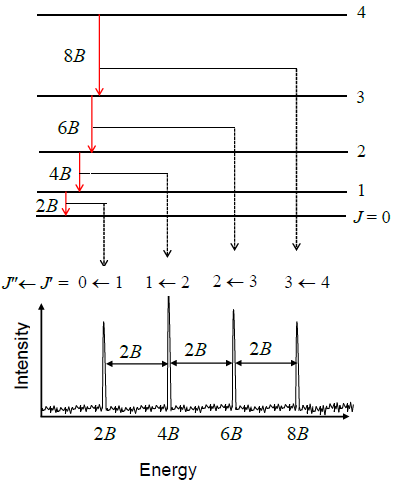
\includegraphics[width=100mm]{1_HW5.png}
		\end{figure}
		
		but since this is what the problem
		asks for, I'll leave $B$ in its unconventional form. 
		\\
		\\
		The inertia of a diatomic molecule can be given in terms of a reduced mass and bond length as
		\[
			I = \mu r_0^2
		\]
		and so $r_0$ can be expressed in terms of $B$ as
		\[
			r_0^2 = \frac{\h^2}{\mu B}.
		\]
		\\
		\item
		At time $t=0$, the molecule is prepared in the superposition state 
		\[
			\psi = \frac{1}{\sqrt 2}\plr{Y_{00}+Y_{10}}.
		\]
		This state evolves to $\psi(t)$ at time $t$. Show that $|\psi(t)|^2$ is a periodic function of time and determine its
		period $T$. 
		\\
		\\
		To find the time dependence, we can apply the time evolution operator 
		\[
			\frac{1}{\sqrt 2}\exp\blr{-\frac i\h Ht}(\ket{0,0}+\ket{1,0}).
		\]
		Since the initial state is a superposition of the eigenfunctions of the Hamiltonian, the time dependence is the simple
		exponential evolution:
		\ba
			\ket{\psi(t)} &=  \frac{1}{\sqrt2}\ket{0,0}+\frac{1}{\sqrt 2}e^{-\frac{i}{\h}\frac{1}{2I}2\h^2t}\ket{1,0}.
		\ea
		The probability amplitude is then
		\ba
			|\braket{\vect x|\psi(t)}|^2 &= \frac{1}{2}|\braket{\vect x|0,0}|^2+\frac{1}{2}|\braket{\vect x|1,0}|^2\\
			&\quad+\frac 12e^{i\omega t}
			\braket{1,0|\vect x}\braket{\vect x|0,0}+\frac 12e^{-i\omega t}\braket{0,0|\vect x}\braket{\vect x|1,0}.
		\ea
		where 
		\[
			\omega = \frac{\h}{I} .
		\]
		In terms of spherical harmonics the probability amplitude is
		\[
			|\psi(t)|^2 = \frac{1}{2}\plr{|Y_{00}|^2+|Y_{10}|^2+e^{i\omega t}Y^*_{10}Y_{00}+e^{-i\omega t}
			Y^*_{00}Y_{10}}
		\]
		and the period of oscillation is
		\[
			T = 2\pi\frac{I}{\h}.
		\]
		\\
		\eenum
		
% #4 ---------------------------------------------------------------------------------------------------------------------------------------------------------------------
	\item
	The angular momentum operators for states with a certain $l$ value can be expressed in a matrix representation as
	\[
		L_x = \frac{\h}{\sqrt 2}\begin{pmatrix}0&1&0\\1&0&1\\0&1&0\end{pmatrix};\ 
		L_y = \frac{\h}{\sqrt 2}\begin{pmatrix}0&-i&0\\i&0&-i\\0&i&0\end{pmatrix};\ 
		L_z = \h\begin{pmatrix}1&0&0\\0&0&0\\0&0&-1\end{pmatrix}.
	\]
	The above matrix elements are defined with respect to an orthonormal basis set 
	$\mathcal{B} = \clr{\ket{\phi_1},\ket{\phi_2},\ket{\phi_3}}$. For example, the $(i,j)^{th}$ element of $L_x$ is
	$\braket{\psi|L_x|\psi}$, with $\braket{\phi_i|\phi_j} = \delta_{ij}\ (i,j = 1,2,3)$. 
	\\
		\benum
		% (a)
		\item
		Identify the $l$ value and a basis $\mathcal B$ appropriate to this matrix representation.
		\\
		\\
		Since there are exactly three basis vectors, $l=1$ and $m = -1,0,1$. The basis is the spherical
		harmonics $\ket{l,m}$
		\[
			\mathcal B = \clr{\ket{1,1},\ket{1,0},\ket{1,-1}}
		\]
		or in position space
		\[
			\mathcal B = \clr{Y_{11}(\theta,\phi),Y_{10}(\theta,\phi),Y_{1-1}(\theta,\phi)}.
		\]
		A quick check on the $L_z$ matrix confirms the basis is also in the correct order.
		\\
		
		% (b)
		\item
		Compute the matrices $L_+$, $L_-$ and $L^2$ in your basis.
		\\
		\\
		First we recall that
		\[
			L_+ = L_x+ iL_y;\quad L_- = L_x-iL_y=L_+^\dag.
		\]
		Therefore we can form $L_\pm$ based on the matrices given. Starting with $L_+$,
		\ba
			L_+ &= \frac{\h}{\sqrt 2}\begin{pmatrix}0&1&0\\1&0&1\\0&1&0\end{pmatrix}
			+\frac{\h}{\sqrt2}i \begin{pmatrix}0&-i&0\\i&0&-i\\0&i&0\end{pmatrix} \\
			&=\frac{\h}{\sqrt 2}\clr{\begin{pmatrix}0&1&0\\1&0&1\\0&1&0\end{pmatrix}
			+\begin{pmatrix}0&1&0\\-1&0&1\\0&-1&0\end{pmatrix}}\\
			& = \frac{2\h}{\sqrt 2}\begin{pmatrix}0&1&0\\0&0&1\\0&0&0\end{pmatrix}.
		\ea
		Using $L_- = L_+^\dag$
		\[
			L_- = \frac{2\h}{\sqrt 2}\begin{pmatrix}0&0&0\\1&0&0\\0&1&0\end{pmatrix}.
		\]
		Lastly we can use
		\[	
			L^2 = \frac{1}{2}(L_+L_-+L_-L_+)+L_z^2 
		\]
		to form $L^2$. Term by term we have
		\ba
			\frac{1}{2}(L_+L_-+L_-L_+) &= \h^2\clr{
			\begin{pmatrix}0&1&0\\0&0&1\\0&0&0\end{pmatrix}
			\begin{pmatrix}0&0&0\\1&0&0\\0&1&0\end{pmatrix}+
			\begin{pmatrix}0&0&0\\1&0&0\\0&1&0\end{pmatrix}
			\begin{pmatrix}0&1&0\\0&0&1\\0&0&0\end{pmatrix}}\\
			& = \h^2\clr{
			\begin{pmatrix}1&0&0\\0&1&0\\0&0&0\end{pmatrix}+
			\begin{pmatrix}0&0&0\\0&1&0\\0&0&1\end{pmatrix}}\\
			& = \h^2
			\begin{pmatrix}1&0&0\\0&2&0\\0&0&1\end{pmatrix}
		\ea
		and
		\[
			L_z^2 = \h^2 \begin{pmatrix}1&0&0\\0&0&0\\0&0&1\end{pmatrix}.
		\]
		Putting them together
		\[
			L^2 = 2\h^2\begin{pmatrix}1&0&0\\0&1&0\\0&0&1\end{pmatrix}.
		\]
		Altogether now,
		\[
			L_+= \frac{2\h}{\sqrt 2}\begin{pmatrix}0&1&0\\0&0&1\\0&0&0\end{pmatrix};\quad
			L_- = \frac{2\h}{\sqrt 2}\begin{pmatrix}0&0&0\\1&0&0\\0&1&0\end{pmatrix};\quad
			L^2 = \h^2\begin{pmatrix}1&0&0\\0&1&0\\0&0&1\end{pmatrix}.
		\]
		We can see that $L^2$ was calculated correctly since it is diagonal with eigenvalues $2\h^2$. 
		\\
		\\
		% (c)
		\item
		For the state $\psi = \frac{1}{\sqrt 2}(\ket{\phi_1}+\ket{\phi_3})$, compute the expectation values
		$\braket{\psi|L_x|\psi}$, $\braket{\psi|L_y|\psi}$ and $\braket{\psi|L_z|\psi}$.
		\\
		\\
		In matrix notation we start with $\braket{\psi|L_x|\psi}$,
		\ba
			\braket{\psi|L_x|\psi} &= 
			\frac{\h}{2\sqrt 2}\begin{pmatrix}1&0&1\end{pmatrix}
			\begin{pmatrix}0&1&0\\1&0&1\\0&1&0\end{pmatrix}
			\begin{pmatrix}1\\0\\1\end{pmatrix}\\
			& = \frac{\h}{2\sqrt 2}
			\begin{pmatrix}0&2&0\end{pmatrix}
			\begin{pmatrix}1\\0\\1\end{pmatrix}\\
			& = 0.
		\ea
		Now for $\braket{\psi|L_y|\psi}$,
		\ba
			\braket{\psi|L_y|\psi} &= 
			\frac{i\h}{2\sqrt 2}\begin{pmatrix}1&0&1\end{pmatrix}
			\begin{pmatrix}0&-1&0\\1&0&-1\\0&1&0\end{pmatrix}
			\begin{pmatrix}1\\0\\1\end{pmatrix}\\
			& = \frac{i\h}{2\sqrt 2}
			\begin{pmatrix}0&0&0\end{pmatrix}
			\begin{pmatrix}1\\0\\1\end{pmatrix}\\
			& = 0.
		\ea
		Lastly
		 $\braket{\psi|L_z|\psi}$,
		\ba
			\braket{\psi|L_z|\psi} &= 
			\frac{\h}{2}\begin{pmatrix}1&0&1\end{pmatrix}
			\begin{pmatrix}1&0&0\\0&0&0\\0&0&-1\end{pmatrix}
			\begin{pmatrix}1\\0\\1\end{pmatrix}\\
			& = \frac \h2 
			\begin{pmatrix}1&0&-1\end{pmatrix}
			\begin{pmatrix}1\\0\\1\end{pmatrix}\\
			& = 0.
		\ea
		Altogether now
		\[
			 \braket{\psi|L_x|\psi} =   \braket{\psi|L_y|\psi} =   \braket{\psi|L_z|\psi} =0.
		\]
		\\
		Do these results make any sense? If we recall the first problem we found that 
		\[
			\braket{l,m|L_x|l,m} = \braket{l,m|L_y|l,m} = 0.
		\]
		As such, any non-zero expectation value can only arise from two differing states. However, if we recall that $L_x$
		and $L_y$ are formed by the sum or difference of raising operators then we can observe that the $L_x$ and $L_y$
		only raise/lower any given state by one level. Since our system is separated by two levels of $m$, the raising/lowering
		operators still produce orthogonal inner products. As for $L_z$, since the two eigenvalues $\h$ and $-\h$ are equal
		and opposite there is cancellation. Had our superposition of states been between adjacent vectors, then we should 
		have a non-zero expectation value for such operators. 
		\\
		\\
		\eenum

		
% #5 -------------------------------------------------------------------------------------------------------------------------------------------------------------------------
	\item 
	Sakurai 3.3: Consider the $2\times2$ matrix defined by
	\[
		U = \frac{a_0+i\vect \sigma\cdot \vect a}{a_0-i\vect \sigma\cdot\vect a},
	\]
	where $a_0$ is a real number and $\vect a$ is a three-dimensional vector with real components. 
	
		\benum
		% (a)
		\item
		Prove that $U$ is unitary and unimodular.
		\\
		\\
		We seek to prove $\det(U) = 1$ and $UU^\dag = U^\dag U = 1$. First note that 
		\[
			\vect \sigma\cdot\vect a = \sum a_i\sigma_i
		\]
		is a $2\times2$ Hermitian matrix, since $\sigma_i = \sigma_i^\dag$. Since $U$ is also a $2\times 2$ matrix we can write 
		it as
		\[
			U = \plr{a_0\mathbb I+i\sigma\cdot\vect a}\plr{a_0\mathbb I-i\sigma\cdot\vect a}^{-1}
		\]
		where $\mathbb I$ is the identity matrix. Further, if we denote
		\[
			A = a_0\mathbb I+i\sigma\cdot\vect a
		\]
		then we can write $U$ as
		\[
			U = A(A^\dag)^{-1}.
		\]
		Let's take the product of $AA^\dag$,
		\ba
			AA^\dag &= (a_0\mathbb I+i\sigma\cdot\vect a)( a_0\mathbb I-i\sigma\cdot\vect a)\\
			& = a_0^2\mathbb I + (\sigma\cdot\vect a)^2\\
			& = (a_0^2 +|\vect a|^2)\mathbb I
		\ea
		where we have used $(\sigma\cdot\vect a)^2 = |\vect a|^2$. Notice that $AA^\dag$ is Hermitian.  Now lets put $A$ and 
		$A^\dag$ n matrix form and find their determinants,
		\[
			A = \begin{pmatrix}a_0+ia_3&a_2+ia_1\\-a_2+ia_1&a_0-ia_3\end{pmatrix}
		\]
		\[
			A^\dag = \begin{pmatrix}a_0+ia_3&-a_2-ia_1\\a_2-ia_1&a_0-ia_3\end{pmatrix}
		\]
		and
		\[
			\det(A) = a_0^2+a_3^2+a_2^2+a_1^2 = a_0^2+|\vect a|^2 = \det(A^\dag).
		\]
		Thus we have discovered that
		 \[
		 	AA^\dag = \mathbb I\det(A) = \mathbb I\det(A^\dag) = A^\dag A
		\]
		so
		\[
			A = \det(A)(A^\dag)^{-1}
		\]
		\[
			(A^\dag)^{-1} = \frac{A}{\det(A)}.
		\]
		Now we can form $U$ as
		\ba
			U &= A(A^\dag)^{-1}\\
			& = \frac{A^2}{\det A}
		\ea
		and so
		\ba
			UU^\dag &= \frac{1}{(\det A)^2}AAA^\dag A^\dag \\
			& = \frac{1}{\det(A)}AA^\dag\\
			& = \mathbb I\\
			& = U^\dag U.
		\ea
		Therefore $U$ is unitary. As for the determinant
		\ba
			\det(U) &= \det\plr{\frac{A^2}{\det(A)}}\\
			&= \frac{\det(A^2)}{\det(A)^2} \\
			& = 1.
		\ea
		Therefore $U$ is also unimodular. 
		\\
		\\
		% (b)
		\item
		In general, a $2\times 2$ unitary unimodular matrix represents a rotation in three dimensions. Find the axis and angle of
		rotation appropriate for $U$ in terms of $a_0,a_1,a_2$, and $a_3$. 
		\\
		\\
		To find the axis and angle of rotation, we seek to cast $U$ into a form that matches the $2\times 2$ representation 
		of the rotation operator. That is
		\[
			\exp\plr{\frac{-i\vect\sigma\cdot\vecth n\phi}{2}} = \mathbb I\cos\pfrac{\phi}{2}-i\vect\sigma\cdot\vecth
			n\sin\pfrac{\phi}{2}.
		\]
		To do so, lets form $U$ as
		\ba
			U& = \frac{A^2}{\det(A)}\\
			& = \frac{1}{\det(A)}(a_0+i\sigma\cdot\vect a)^2\\
			& = \frac{1}{\det(A)}\plr{a_0^2+2ia_0(\sigma\cdot\vect a) - |\vect a|^2}\\
			& = \plr{\frac{a_0^2-|\vect a|^2}{a_0^2+|\vect a|^2} }-i\sigma\cdot\vecth a\pfrac{-2a_0|\vect a|}{a_0^2+|\vect a|^2}.
		\ea
		In this form it is clear to see that
		\[
			 \vecth n = \vecth a
		\]
		\[
			\cos\pfrac{\phi}{2} = \frac{a_0^2-|\vect a|^2}{a_0^2+|\vect a|^2}
		\]
		\[
			\sin\pfrac{\phi}{2} = \frac{-2a_0|\vect a|}{a_0^2+|\vect a|^2}.
		\]
		\\	
		\eenum
		
		
% #6 ------------------------------------------------------------------------------------------------------------------------------------------------------------------------
	\item 
	Sakurai 3.17: The wave function of a particle subjected to a spherically symmetric potential $V(r)$ is given by
	\[
		\psi(\vect x) = (x+y+3z)f(r).
	\]
	
		\benum
		% (a)
		\item
		Is $\psi$ an eigenfunctions of $\vect L^2$? If so, what is the $l$-value? If not, what are the possible values of 
		$l$ that we may obtain when $\vect L^2$ is measured?
		\\
		\\
		\\
		To check to see if $\psi(\vect x)$ is an eigenfunction of $\vect L^2$, we will simply need to convert it to polar 
		coordinates and apply $\vect L^2$. As such
		\[
			\psi(r,\theta,\phi) = rf(r)(\sin\theta\cos\phi+\sin\theta\sin\phi+3\cos\theta).
		\]
		Applying $\vect L^2$, 
		\ba
			 &-\h^2\blr{\frac{1}{\sin\theta}\pdiff\theta\plr{\sin\theta\pdiff\theta}+\frac{1}{\sin^2\theta}\pdifff{}{*2\phi}}
			 \psi(r,\theta,\phi)\\
			 =& -\h^2rf(r)\blr{\frac{1}{\sin\theta}\pdiff\theta\plr{\sin\theta\pdiff\theta}+\frac{1}{\sin^2\theta}\pdifff{}{*2\phi}}
			 (\sin\theta\cos\phi+\sin\theta\sin\phi+3\cos\theta).
		\ea
		Term by term
		\ba
			 \frac{1}{\sin^2\theta}\pdifff{}{*2\phi}  &(\sin\theta\cos\phi+\sin\theta\sin\phi+3\cos\theta) \\
			=&- \frac{1}{\sin^2\theta}(\sin\theta\cos\phi+\sin\theta\sin\phi )\\
			=&-\frac{1}{\sin\theta}(\cos\phi+\sin\phi)
		\ea
		\ba
			\frac{1}{\sin\theta}\pdiff\theta\plr{\sin\theta\pdiff\theta}&(\sin\theta\cos\phi+\sin\theta\sin\phi+3\cos\theta)\\
			=&\frac{1}{\sin\theta}\pdiff\theta\sin\theta(\cos\theta\cos\phi+\cos\theta\sin\phi-3\sin\theta)\\
			=&\frac{1}{\sin\theta}\blr{(\cos^2\theta-\sin^2\theta)(\cos\phi+\sin\phi)-6\sin\theta\cos\theta}\\
			=&\frac{1}{\sin\theta}(\cos(2\theta)(\cos\phi+\sin\phi)-3\sin(2\theta)).
		\ea
		Adding them together we have
		\ba
			\blr{\frac{1}{\sin\theta}\pdiff\theta\plr{\sin\theta\pdiff\theta}+\frac{1}{\sin^2\theta}\pdifff{}{*2\phi}}&
			 (\sin\theta\cos\phi+\sin\theta\sin\phi+3\cos\theta) \\ &=\frac{1}{\sin\theta}
			 \blr{(\cos(2\theta)-1)(\cos\phi+\sin\phi)-3\sin(2\theta)}\\
			 & = -2(\sin\theta\cos\phi+\sin\theta\sin\phi+3\cos\theta).
		\ea
		Now we can see that
		\[
			\vect L^2 \psi(r,\theta,\phi) = 2\h^2 \psi(r,\theta,\phi).
		\]
		Therefore we deduce that $l=1$! 
		\\
		\\
		% (b)
		\item
		What are the probabilities for the particle to be found in various $m_l$ states?
		\\
		\\
		Since the wavefunction has been determined for $l=1$, we expect it to be composed of a linear combination of
		the three possible states corresponding to $m=-1,0,1$. Thus we can write
		\[
			\psi(\vect x) = rf(r)g(\theta,\phi) = rf(r)\sum_{m}c_m Y_1^m(\theta,\phi).
		\] 
		The task is then to decompose $g(\theta,\phi)$ as a sum of spherical harmonics. The three harmonics we need are
		\[
			Y_1^{-1} = \sqrt{\frac{3}{8\pi}}\sin\theta e^{-i\phi};\quad 
			Y_1^0 = \sqrt{\frac{3}{4\pi}}\cos\theta;\quad 
			Y_1^1 = \sqrt{\frac{3}{8\pi}}\sin\theta e^{i\phi}.
		\]
		Using these, we express our wavefunction as
		\ba
			\psi(\vect x) &= rf(r)\blr{\sin\theta\plr{\frac{e^{i\phi}+e^{-i\phi}}{2}+\frac{e^{i\phi}-e^{-i\phi}}{2i}}+3\cos\theta}\\
			& = rf(r)\blr{\frac{1}{2}(1-i)\sin\theta e^{i\phi}+\frac 12(1+i)\sin\theta e^{-i\phi}+3\cos\theta}\\
			& = rf(r)\blr{-\sqrt{\frac{2\pi}{3}}(1-i)Y_1^1+\sqrt{\frac{2\pi}{3}}(1+i)Y^{-1}_1+2\sqrt{3\pi}Y_1^0}.
		\ea
		As the wavefunction is not normalized, we can find the probabilities as
		\[	
			P_m = \frac{|c_m|^2}{\sum|c_m|^2}.
		\]
		For the coefficients we have
		\[
			|c_{-1}|^2 = |c_1|^2 =  \frac{4\pi}{3};\quad |c_0|^2 = 12\pi.
		\]
		Since only the ratio of probabilities is important, we can pull out a factor of $\frac{4\pi}{3}$ to obtain
		\[
			|c_{-1}|^2 = |c_1|^2 =  1;\quad |c_0|^2 = 9
		\]
		and thus
		\[
			P_{-1} = P_{1} = \frac{1}{11};\quad P_0 = \frac{9}{11}
		\]
		\\
		\\
		% (c)
		\item
		Suppose it is known somehow that $\psi(\vect x)$ is an energy eigenfunction with eigenvalue $E$. Indicate how 
		we may find $V(r)$. 
		\\
		\\
		Since the $\vect L^2$ operator in position space is just the angular part of the Laplacian, we can express the Laplacian
		in spherical coordinates as
		\[
			\del^2 = \frac{1}{r^2}\pdiff r \plr{r^2\pdiff r}+\frac{\vect L^2}{r^2}.
		\]
		In addition, we can write any spherically symmetric Hamiltonian as
		\[
			H = \frac{\vect p^2}{2m}+V(r) .
		\]
		Therefore, the time independent Schrodinger equation is then
		\[
			\blr{-\frac{\h^2}{2mr^2}\pdiff r \plr{r^2\pdiff r}+\frac{\vect L^2}{2mr^2}+V(r)}\psi(\vect x) = E\psi(\vect x).
		\]
		Now, we already know how $\vect L^2$ affects $\psi(\vect x)$ (being an eigenvector) and we are assuming the
		$\psi(\vect x)$ is an energy eigenfunction. Therefore we can write the TISE as
		\[
			  \blr{-\frac{\h^2}{2mr^2}\pdiff r \plr{r^2\pdiff r}+\frac{2\h^2}{2mr^2}-E}\psi(\vect x) = V(r)\psi(\vect x).
		\]
		Inputting the explicit form of $\psi(\vect x)$ we find
		\[
			-\frac{\h^2}{2mr^2}\pdiff r \plr{r^2\pdiff r}rf(r)g(\theta,\phi) 
			+rf(r)g(\theta,\phi)\plr{\frac{\h^2}{mr^2}-E} = -V(r)rf(r)g(\theta,\phi).
		\]
		We can solve part of the first term as
		\[
			\pdiff r \plr{r^2\pdiff r}rf(r)g(\theta,\phi)  =r[r^2f''(r)+4rf'(r)+2f(r)]g(\theta,\phi) .
		\]
		Substituting this in we find
		\ba
				-\frac{\h^2}{2mr^2}r[r^2f''(r)+4rf'(r)+2f(r)]g(\theta,\phi)
			+rf(r)g(\theta,\phi)\plr{\frac{\h^2}{mr^2}-E} \\= -V(r)rf(r)g(\theta,\phi).
		\ea
		The third and fourth terms cancel! In addition we can eliminate $g(\theta,\phi)$. Then we have
		\[
			-\frac{\h^2}{2mr^2}[f''(r)+4rf'(r)]- Ef(r) = -V(r)f(r)
		\]
		and thus the potential can finally be expressed as
		\[
			V(r) = \frac{\h^2}{2mr}\frac{rf''(r)+4f'(r)}{f(r)}+E.
		\]
		
		\eenum
		
% #7 ------------------------------------------------------------------------------------------------------------------------------------------------------------------------
	\item
	Sakura 3.20: Consider an orbital angular-momentum eigenstate $\ket{l=2,m=0}$. Suppose this state is rotated by an angle
	$\beta$ about the $y$-axis. Find the probability for the new state to be found in $m=0,\pm1$, and $\pm2$. (The spherical 
	harmonics for $l=0,1$ and $2$ given in Section B.5 in Appendix B may be useful.)
	\\
	\\
	\\
	To rotate the state $\ket{2,0}$ by an angle $\beta$ about the $y$-axis is to apply the rotation operator to the our state
	\[
		\ket{2,0}_R = \exp\blr{-\frac{i}{\h}J_y\beta}\ket{2,0}.
	\]
	The expectation value to find this state in a state of a given $m$ (since $l$ does not change under rotation) is
	\[
		\braket{2,m|\exp\blr{-\frac{i}{\h}J_y\beta}|2,0}.
	\]
	These expectation values we seek can be observed to be members of the Wigner functions defined by
	\[
		\mathcal D_{m'm}^{j}(R) = \braket{j,m'|\exp\blr{-\frac i\h \vect J\cdot\vecth n\phi}|j,m}.
	\]
	where we use the $j=2=l$ space. It turns out that these Wigner functions for orbital angular momentum that we need
	 are closely related to the spherical harmonics and we can use Sakurai eq 3.6.52 as
	\[
		\mathcal D_{m0}^2(\beta) = \sqrt{\frac{4\pi}{(2l+1)}}Y_2^{m*}(\beta,0).
	\]
	Now we compose the Wigner functions we need:
	\ba
		\mathcal D_{-20}^2(\beta) &=\sqrt{\frac{3}{8}}\sin^2\beta\\
		\mathcal D_{-10}^2(\beta) &=\sqrt{\frac{3}{2}}\sin\beta\cos\beta\\
		\mathcal D_{00}^2(\beta) &= \frac{1}{2}(3\cos^2\beta-1)\\
		\mathcal D_{10}^2(\beta) &= -\sqrt{\frac{3}{2}}\sin\beta\cos\beta\\
		\mathcal D_{20}^2(\beta) &= \sqrt{\frac{3}{8}}\sin^2\beta
	\ea	
	where we saved some work by using the relationship between positive and negative $m$ of the spherical 
	harmonics. Lastly, to find the probabilities $P_m$ at different values of $m$, we take the modulus squared:
	\ba
		P_{0} &= \frac{3}{8}\sin^4\beta\\
		P_{\pm 1} &= \frac{3}{2}\sin^2\beta\cos^2\beta\\
		P_{\pm 2} &= \frac{1}{4}(3\cos^2\beta-1)^2.
	\ea
	If we like, we could take the sum of these probabilities to verify that they add to unity; however, playing around with trig. functions
	right now does not sound very fun. 
	\\
	\\
% #8 ---------------------------------------------------------------------------------------------------------------------------------------------------------------------
	\item 
	The goal of this problem is to determine the degenerate eigenstates of the three dimensional isotropic harmonic oscillator written
	as eigenstates of $\vect L^2$ and $L_z$, in terms of Cartesian eigenstates $\ket{n_xn_yn_z}$. 
	
	\benum
	% (a)
	\item
	Show that the angular-momentum operators are given by
	\[
		L_i = i\h \epsilon_{ijk}a_ja_k^\dag
	\]
	\[
		\vect L^2 = \h^2\blr{N(N+1)-a_k^\dag a_k^\dag a_ja_j},
	\]
	where summation is implied over repeated indices, $\epsilon_{ijk}$ is the totally antisymmetric symbol, and $N\equiv a_j^\dag
	a_j$ counts the total number of quanta.
	\\
	\\
	As the $a_i$ represent the familiar raising and lowering operators in one dimension, a sensible first step to constructing the
	relation for $L_i$ may be to express the angular momentum in terms of $\vect x$ and $\vect p$ and then substitute the
	creation/annihilation operators as necessary. Starting with the cross product,
	\[	
		\vect L = \vect x\times \vect p 
	\]
	we have for each element
	\[
		L_i = \epsilon_{ijk}x_jp_k.
	\]
	We can write it in this form (Einstein notation implied) without worrying about commutation because $[x_j,p_k] = i\h\delta_{jk}$. 
	Going back to the 1D harmonic oscillator we recall
	\[
		a_i = \sqrt{\frac{m\omega}{2\h}}\plr{x_i+\frac{ip_i}{m\omega}},\quad a_i^\dag = \sqrt{\frac{m\omega}{2\h}}
		\plr{x_i-\frac{ip_i}{m\omega}}.
	\]
	Now we evaluate
	\[
		a_ja^\dag_k  = \frac{m\omega}{2\h}\plr{x_jx_k+\frac{1}{(m\omega)^2}p_jp_k- \frac{i}{m\omega}(x_jp_k-p_jx_k)}.
	\]
	Including the Levi-Civita and constant in front we have (for fixed $i$)
	\ba
		i\h\epsilon_{ijk}a_ja^\dag_k &=  \frac{-m\omega}{2}\plr{(x_jx_k-x_kx_j)
		+\frac{1}{(m\omega)^2}(p_jp_k-p_kp_j)}\\
		&\quad\frac{1}{2}\blr{(x_jp_k-p_jx_k)-(x_kp_j-p_kx_j)}\\
		&= \frac{1}{2}\blr{(x_jp_k-p_jx_k)+(p_kx_j-x_kp_j)}\\
		& = \frac{1}{2}\plr{[x_j,p_k]+2p_kx_j-([p_j,x_k]+2x_kp_j)}\\
		& = \frac{1}{2}\plr{2i\h\delta_{jk}+2(p_kx_j-x_kp_j)}\\
		& = p_kx_j-x_kp_j\\
		& = \epsilon_{ijk}x_jp_k.
	\ea
	Therefore we see that
	\[
		L_i = i\h\epsilon_{ijk}a_ja_k^\dag = \epsilon_{ijk}x_jp_k.
	\]
	\\
	Moving onto the $\vect L^2$ operator, we have
	\ba
		\vect L^2 &= L_i^{i2} = \sum_i L_i^2\\
		& = \sum_i -\h^2 (\epsilon_{ijk}a_ja_k^\dag)^2\\
		& =  -\h^2\clr{(a_ja_k^\dag-a_ka^\dag_j)^2+(a_ka_i^\dag-a_ia_k^\dag)^2+(a_ia_j^\dag-a_ja_i^\dag)^2}.
	\ea
	In this notation, we are now holding the indices fixed (no einstein summation). If we expand the first term we have
	\be\label{2}
			(a_ja_k^\dag-a_ka_j^\dag)^2 = a_ja_k^\dag a_ja_k^\dag -a_ja_k^\dag a_ka_j^\dag-a_ka_j^\dag a_ja_k^\dag
		 +a_ka_j^\dag a_ka_j^\dag.
	\ee
	If we recall the commutation relations 
	\[
		[a_i,a_j] = 0, \quad [a_i,a_j^\dag] = \delta_{ij}
	\]
	then we can see that we are allowed to swap any two operators with the exception that they are the same index and 
	hermitian conjugates (cannot swap $a_j^\dag a_j$). As such we can reform \eqref 2 as
	\[
			(a_ja_k^\dag-a_ka_j^\dag)^2=
			 a_k^\dag a_k^\dag a_ja_j +
			 a_j^\dag a_j^\dag a_ka_k - 
			 a_k^\dag a_k a_j a_j^\dag -
			 a_j^\dag a_j a_k a_k^\dag.
	\]
	In addition, we can also use the commutation relation 
	\[
		a_ia_i^\dag = a_i^\dag a_i + 1
	\]
	in which we can partially form the number operator as
	\[
		a_ia_i^\dag = N_{ii} +1 
	\]
	where we denote
	\[
		\sum_i N_{ii} = \sum_i a_i^\dag a_i = N .
	\]
	Making these substitutions, our first term  \eqref 2 we have been dealing with becomes
	\[
			(a_ja_k^\dag-a_ka_j^\dag)^2=
			 a_k^\dag a_k^\dag a_ja_j +
			 a_j^\dag a_j^\dag a_ka_k - 
			 N_{kk}(N_{jj}+1) -
			N_{jj}(N_{kk}+1).
	\]
	If we now take the sum of all three quadratic terms ($L_1^2+L_2^2+L_3^3$) we can write our final answer in Einstein
	summation notation as
	\[
		\vect L^2 = \h^2\blr{N(N+1)-a_k^\dag a_k^\dag a_ja_j}.
	\]
	However, there is one detail we left out - we did not find any terms with all identical indices when we expanded 
	the $L_i^2$ components. And the $\vect L^2$  we just wrote down  must sum over \emph{all} indices, including those that are the 
	same. To solve this dilemma, all we have to do is take a glance at \eqref 2 and set the indices to be the same $j=k$. It is then 
	apparent that the result is zero and therefore the same index sums make no contribution to $\vect L^2$. So it is in fact safe to write it 
	in this Einstein convention after all. 
	\\
	\\
	\emph{If one made proper use of the Levi-Civita tensor, I assume there may be a more elegant and robust way to solve this 
	problem? }
	\\
	\\

	% (b)
	\item
	Use these relations to express the states $\ket{qlm} =\ket{01m}$, $m=0,\pm1$, in terms of the three eigenstates $\ket{n_xn_yn_z}$
	that are degenerate in energy. Write down the representation of your answer in coordinate space, and check that the 
	angular and radial dependencies are correct.
	\\
	\\
	The three degenerate angular momentum eigenstates $\ket{q,l,m}$ are
	\[ 
		\ket{0,1,-1},\quad\ket{0,1,0},\quad\ket{0,1,1}
	\]
	while the three degenerate cartesian eigenstates $\ket{n_x,n_y,n_z}$ are
	\[
		\ket{1,0,0},\quad\ket{0,1,0}\quad\ket{0,0,1}.
	\]
	Both set of states are orthogonal and complete (for a single energy) and serve as energy eigenkets to the harmonic oscillator 
	Hamiltonian. Our task is to find the transformation matrix that relates these states to each other. We can express an angular 
	momentum state as the linear superposition of cartesian states
	\ba
		\ket{0,1,m} &= \braket{1,0,0|0,1,m}\ket{1,0,0}+\braket{0,1,0|0,1,m}\ket{0,1,0}\\
		&\quad + \braket{0,0,1|0,1,m}\ket{0,0,1}.
	\ea
	The inner products represents the usual probability of state overlap, and these are the complex coefficients we seek. We can 
	denote them as $c_{I'm}$ and write the expansion of the angular momentum state as
	\[
		\ket{0,1,m} = c_{1m}\ket{1,0,0}+c_{2m}\ket{0,1,0}+c_{3m}\ket{0,0,1}.
	\]
	In matrix notation, this would form a $3\times3$ unitary transformation matrix. To find these elements, one possible avenue may 
	be to compute the effects of various angular momentum operators on both the angular momentum eigenstates and the cartesian
	eigenstates. 
	\\
	\\
	Let's first look at $\vect L^2$. On the angular momentum state we have
	\[
		\vect L^2\ket{0,1,m} = 2\h^2\ket{0,1,m}
	\]
	while for the cartesian states we have
	\ba
		\vect L^2&( c_{1m}\ket{1,0,0}+c_{2m}\ket{0,1,0}+c_{3m}\ket{0,0,1}) \\
		&=  \h^2\blr{N(N+1)-a_k^\dag a_k^\dag a_ja_j}
		( c_{1m}\ket{1,0,0}+c_{2m}\ket{0,1,0}+c_{3m}\ket{0,0,1}) \\
		&= 2\h^2( c_{1m}\ket{1,0,0}+c_{2m}\ket{0,1,0}+c_{3m}\ket{0,0,1}) .
	\ea
	Notice that the operator $a_k^\dag a_k^\dag a_ja_j$ has no effect on our cartesian states since no state can be lowered twice. 
	No new information is really gained from application of $\vect L^2$. 
	\\
	\\
	Next we apply $L_z$, defined in cartesian operators as
	\[
		L_z = i\h(a_xa_y^\dag-a_ya_x^\dag).
	\]
	For the angular state we have
	\[
		L_z\ket{0,1,m} = m\h\ket{0,1,m} 
	\]
	while for the cartesian states we have
	\ba
		L_z &( c_{1m}\ket{1,0,0}+c_{2m}\ket{0,1,0}+c_{3m}\ket{0,0,1}) \\
		&=i\h(a_xa_y^\dag-a_ya_x^\dag)(c_{1m}\ket{1,0,0}+c_{2m}\ket{0,1,0}+c_{3m}\ket{0,0,1})\\
		& = i\h( c_{1m}\ket{0,1,0}-c_{2m}\ket{1,0,0}) .
	\ea
	Notice that the cartesian $\ket{0,0,1}$ state has disappeared. Alternatively, we can view this as
	\[
		L_z\ket{0,0,1} = 0.
	\]
	This turns out to be useful information because we also know that when we apply $L_z$ to angular momentum state $m=0$
	we have
	\[
		L_z\ket{0,1,0} = 0.
	\]
	Therefore we can conclude that the angular momentum state $m=0$ is equal to the $n_z=1$ cartesian state
	\[
		\ket{0,1,0} = \ket{0,0,1}.
	\]
	The overlap coefficient $c_{30}$ is unity in this case since both sets of states are normalized. In order to find $c_{1m}$ and
	$c_{2m}$ we will need to look at specific cases of the $z$-component of angular momentum. Starting with angular state
	$\ket{0,1,1}$ (which has no component of cartesian $\ket{0,0,1}$) we have
	\[
		L_z\ket{0,1,1} = \h\ket{0,1,1},
	\]
	while for the cartesian states we have
	\[
		L_z( c_{11}\ket{1,0,0}+c_{21}\ket{0,1,0}) = i\h( c_{11}\ket{0,1,0}-c_{21}\ket{1,0,0}) .
	\]
	Since this state must be an eigenstate we have the relation
	\[
		\h(c_{11}\ket{1,0,0}+c_{21}\ket{0,1,0}) = i\h(c_{11}\ket{0,1,0}-c_{21}\ket{1,0,0}).
	\]
	Equating the coefficients we arrive at
	\[
		c_{11} = -ic_{21},\quad c_{21} = ic_{11}.
	\]
	If we include this with the normalization condition
	\[
		|c_{11}|^2+|c_{21}|^2 = 1
	\]
	we have
	\[
		c_{11} = \frac{1}{\sqrt 2},\quad c_{21} = \frac{i}{\sqrt 2}.
	\]
	Here we have specifically chosen $c_{11}$ to be real - if we desired to, we could have chosen $c_{21}$ to be real instead because 
	the phase will ultimately have no physical impact on the state. If we precede in this same fashion for the angular state
	$\ket{0,1,-1}$ we find that
	\[
		c_{1-1} = \frac{1}{\sqrt 2},\quad c_{2-1} = -\frac{i}{\sqrt 2}.
	\]
	As a quick measure to see if these coefficients are correct we can form the orthogonal inner product of angular states
	\[
		\braket{0,1,1|0,1,-1} = 0
	\]
	in terms of cartesian base kets
	\[
		\plr{\frac{1}{\sqrt 2}\bra{1,0,0}-\frac{i}{\sqrt 2}\bra{0,1,0}}\plr{\frac{1}{\sqrt 2}\ket{1,0,0}-\frac{i}{\sqrt 2}\ket{0,1,0}}.
	\]
	By inspection we see that they are indeed orthogonal. All together we have the relationship between angular
	momentum eigenstates and cartesian eigenstates of the isotropic harmonic oscillator Hamiltonian as 
	\[
		\begin{pmatrix}a_1\\a_2\\a_3\end{pmatrix} = 
		\begin{pmatrix}\frac{1}{\sqrt 2}&\frac{-i}{\sqrt 2}&0
			\\\frac{1}{\sqrt 2}&\frac{i}{\sqrt 2}&0\\
			0&0&1
		\end{pmatrix}
		\begin{pmatrix}b_1\\b_2\\b_3\end{pmatrix}\quad\to\quad A = UB
	\]
	where $A$ is a column matrix composed of angular momentum eigenstates in descending $m$ order and $B$
	is a column matrix descending as $n_x$, $n_y$, and $n_z$. 
		
	% (c)
	\item
	Repeat for $\ket{qlm} = \ket{200}$.
	
	% (d)
	\item
	Repeat for $\ket{qlm} = \ket{02m}$, with $m=0,1$ and $2$. 
	
	\eenum
\eenum
\end{document}